\section{Pilcheur Gamont}

\begin{center}
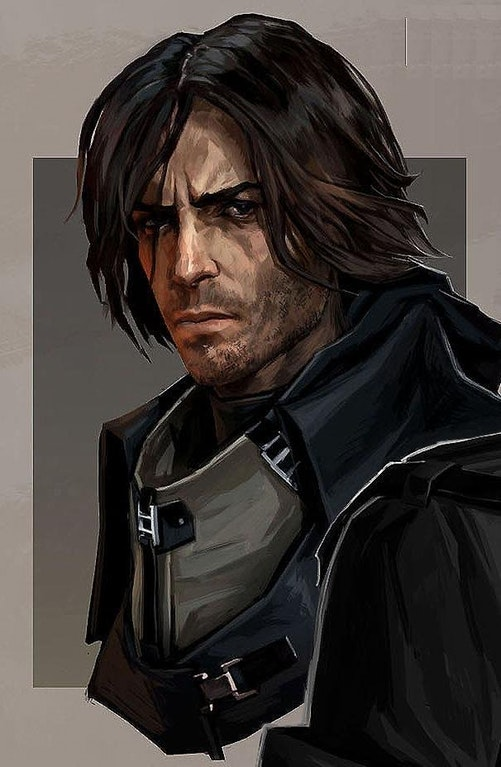
\includegraphics[width=80mm]{./content/img/pilch1.jpg}
\begin{figure}[h]
\end{figure}
\end{center}

\subsection*{Details}

\noindent

Race: 	Human \\
Class: 	Book Burner \\
Age: 	46 \\
Status: Deceased

\subsubsection{Background}

Pilcheur ``Pilch'' Gamont was a Book Burner --- a member of the Church's now-defunct order tasked with hunting down and destroying heretical texts.  A cloaked man dashing over rooftops with a half-burnt tome under one arm, Pilch was killed by mercenaries during a chase across the rooftops of Hope's Rest before being resurrected by Lazarus.

In life, Pilch was already a conflicted figure.  He possessed a deep knowledge of the Church's inner workings, its communication channels, and its dark secrets.  It was later revealed that Pilch had been secretly selling books he was supposed to burn --- a betrayal that contributed to the Church's purge of the entire Book Burner organisation.

\subsubsection{Personality and Traits}

Pilch was the group's most polarising member.  Cowardly in battle yet occasionally brilliant in negotiation, he had a talent for making terrible situations worse and then somehow surviving the fallout.  His relationship with the supernatural was uniquely troubled --- possessed by dark forces early in the campaign, he manifested shadow powers including clouds of magical darkness, a spectral wolf companion (Howlov), and a sentient shadow sword.

Known to the goblins as ``Fishy'', ``Fishwank'', or ``Pilchard'', he was the frequent target of Kolo's pickpocketing and Exme's withering contempt.  Despite this, moments of genuine connection emerged --- Pilch once saved Kolo's life in battle, prompting Kolo to note ``I never knew he cared''.

His various aliases included Papa Lazarizz, and he had a tendency to adopt elaborate (and unconvincing) disguises involving blackface and Jamaican accents.

\subsubsection{Relationships}

Pilch's relationship with the group was defined by mutual distrust tempered by grudging necessity.  Otoria once pinned him against a wall with her greatsword after he murdered a prisoner, warning him: ``You will not do that again''.  Kolo stole from him relentlessly.  Riphard alternated between alliance and attempted drowning.

His familiar, Quoth the Raven, was one of the group's most useful assets despite Kolo's repeated attempts to kill it.  Pilch also maintained connections to his former Book Burner colleagues, including Lillian (a half-elf who ``actually liked fishy'') and the gnome Zippy.

Pilch had a complicated connection to the god Synne, bearing the Mark of Synne on his body --- a divine brand that granted him dark powers but at a terrible cost.

\subsubsection{Pilch's Story}

From his resurrection onward, Pilch struggled to control the dark powers growing within him.  His possession worsened in Riverfall, where the group had to exorcise him using a combination of Riphard's pastoral chanting, Kolo's Killepitsch liquor, and copious vomiting.  The exorcism left him with his shadow sword and a tenuous grip on his darker nature.

Pilch served as the group's reluctant expert on Church operations, helping them establish themselves in Hope's Rest by leveraging his knowledge of guild politics and mercenary contracts.  He helped secure the old Book Burners headquarters as the Gary Guild's base of operations.

Pilch met his end during a sea voyage, taken by a creature of the deep.  His death left the group without their most knowledgeable member on Church matters --- and, despite everything, genuinely mourned by those who had spent so long mocking him.

\clearpage
